%File: anonymous-submission-latex-2026.tex
\documentclass[letterpaper]{article} % DO NOT CHANGE THIS
\usepackage[submission]{aaai2026}  % DO NOT CHANGE THIS
\usepackage{times}  % DO NOT CHANGE THIS
\usepackage{helvet}  % DO NOT CHANGE THIS
\usepackage{courier}  % DO NOT CHANGE THIS
\usepackage[hyphens]{url}  % DO NOT CHANGE THIS
\usepackage{graphicx} % DO NOT CHANGE THIS
\urlstyle{rm} % DO NOT CHANGE THIS
\def\UrlFont{\rm}  % DO NOT CHANGE THIS
\usepackage{natbib}  % DO NOT CHANGE THIS AND DO NOT ADD ANY OPTIONS TO IT
\usepackage{caption} % DO NOT CHANGE THIS AND DO NOT ADD ANY OPTIONS TO IT
\frenchspacing  % DO NOT CHANGE THIS
\setlength{\pdfpagewidth}{8.5in} % DO NOT CHANGE THIS
\setlength{\pdfpageheight}{11in} % DO NOT CHANGE THIS
%
% These are recommended to typeset algorithms but not required. See the subsubsection on algorithms. Remove them if you don't have algorithms in your paper.
\usepackage{algorithm}
\usepackage{algorithmic}
\usepackage{amsmath}
\usepackage{amssymb}
\usepackage{bm}

%
% These are are recommended to typeset listings but not required. See the subsubsection on listing. Remove this block if you don't have listings in your paper.
\usepackage{newfloat}
\usepackage{listings}
\DeclareCaptionStyle{ruled}{labelfont=normalfont,labelsep=colon,strut=off} % DO NOT CHANGE THIS
\lstset{%
	basicstyle={\footnotesize\ttfamily},% footnotesize acceptable for monospace
	numbers=left,numberstyle=\footnotesize,xleftmargin=2em,% show line numbers, remove this entire line if you don't want the numbers.
	aboveskip=0pt,belowskip=0pt,%
	showstringspaces=false,tabsize=2,breaklines=true}
\floatstyle{ruled}
\newfloat{listing}{tb}{lst}{}
\floatname{listing}{Listing}
%
% Keep the \pdfinfo as shown here. There's no need
% for you to add the /Title and /Author tags.
\pdfinfo{
/TemplateVersion (2026.1)
}

% DISALLOWED PACKAGES
% \usepackage{authblk} -- This package is specifically forbidden
% \usepackage{balance} -- This package is specifically forbidden
% \usepackage{color (if used in text)
% \usepackage{CJK} -- This package is specifically forbidden
% \usepackage{float} -- This package is specifically forbidden
% \usepackage{flushend} -- This package is specifically forbidden
% \usepackage{fontenc} -- This package is specifically forbidden
% \usepackage{fullpage} -- This package is specifically forbidden
% \usepackage{geometry} -- This package is specifically forbidden
% \usepackage{grffile} -- This package is specifically forbidden
% \usepackage{hyperref} -- This package is specifically forbidden
% \usepackage{navigator} -- This package is specifically forbidden
% (or any other package that embeds links such as navigator or hyperref)
% \indentfirst} -- This package is specifically forbidden
% \layout} -- This package is specifically forbidden
% \multicol} -- This package is specifically forbidden
% \nameref} -- This package is specifically forbidden
% \usepackage{savetrees} -- This package is specifically forbidden
% \usepackage{setspace} -- This package is specifically forbidden
% \usepackage{stfloats} -- This package is specifically forbidden
% \usepackage{tabu} -- This package is specifically forbidden
% \usepackage{titlesec} -- This package is specifically forbidden
% \usepackage{tocbibind} -- This package is specifically forbidden
% \usepackage{ulem} -- This package is specifically forbidden
% \usepackage{wrapfig} -- This package is specifically forbidden
% DISALLOWED COMMANDS
% \nocopyright -- Your paper will not be published if you use this command
% \addtolength -- This command may not be used
% \balance -- This command may not be used
% \baselinestretch -- Your paper will not be published if you use this command
% \clearpage -- No page breaks of any kind may be used for the final version of your paper
% \columnsep -- This command may not be used
% \newpage -- No page breaks of any kind may be used for the final version of your paper
% \pagebreak -- No page breaks of any kind may be used for the final version of your paperr
% \pagestyle -- This command may not be used
% \tiny -- This is not an acceptable font size.
% \vspace{- -- No negative value may be used in proximity of a caption, figure, table, section, subsection, subsubsection, or reference
% \vskip{- -- No negative value may be used to alter spacing above or below a caption, figure, table, section, subsection, subsubsection, or reference

\setcounter{secnumdepth}{0} %May be changed to 1 or 2 if section numbers are desired.

% Custom macros
\newcommand{\bxi}{\boldsymbol{\xi}}
\newcommand{\bx}{\bm{x}}
\newcommand{\avg}[1]{\langle #1 \rangle}
\newcommand{\e}{{\mathrm{e}}}
\newcommand{\dd}{{\mathrm{d}}}
% \newcommand{\Bnet}{\beta_{\mathrm{net}}}
\newcommand{\Bnet}{\beta}
\newcommand{\phieq}{\phi_{\mathrm{eq}}}
\newcommand{\fret}{f_{\mathrm{ret}}}
\newcommand{\gmax}{g_{\max}}
\newcommand{\acGauss}{\alpha_c^{\mathrm{G}}}
\newcommand{\acBd}{\alpha_c^{\mathrm{bd}}}
\newcommand{\acSd}{\alpha_c^{\mathrm{sd}}}
\newcommand{\acSp}{\alpha_c^{\mathrm{sp}}}
\newcommand{\p}{\partial}
\newcommand{\cas}{\textstyle\frac}


% The file aaai2026.sty is the style file for AAAI Press
% proceedings, working notes, and technical reports.
%

% Title

% Your title must be in mixed case, not sentence case.
% That means all verbs (including short verbs like be, is, using,and go),
% nouns, adverbs, adjectives should be capitalized, including both words in hyphenated terms, while
% articles, conjunctions, and prepositions are lower case unless they
% directly follow a colon or long dash
\title{\bfseries Thermodynamic approach and Saddle-Dominated Capacity
of the LSE Dense Associative Memory}

\author{
    %Authors
    % All authors must be in the same font size and format.
    Written by AAAI Press Staff\textsuperscript{\rm 1}\thanks{With help from the AAAI Publications Committee.}\\
    AAAI Style Contributions by Pater Patel Schneider,
    Sunil Issar,\\
    J. Scott Penberthy,
    George Ferguson,
    Hans Guesgen,
    Francisco Cruz\equalcontrib,
    Marc Pujol-Gonzalez\equalcontrib
}
\affiliations{
    %Afiliations
    \textsuperscript{\rm 1}Association for the Advancement of Artificial Intelligence\\
    % If you have multiple authors and multiple affiliations
    % use superscripts in text and roman font to identify them.
    % For example,

    % Sunil Issar\textsuperscript{\rm 2},
    % J. Scott Penberthy\textsuperscript{\rm 3},
    % George Ferguson\textsuperscript{\rm 4},
    % Hans Guesgen\textsuperscript{\rm 5}
    % Note that the comma should be placed after the superscript

    1101 Pennsylvania Ave, NW Suite 300\\
    Washington, DC 20004 USA\\
    % email address must be in roman text type, not monospace or sans serif
    proceedings-questions@aaai.org
%
% See more examples next
}

%Example, Single Author, ->> remove \iffalse,\fi and place them surrounding AAAI title to use it
\iffalse
\title{My Publication Title --- Single Author}
\author {
    Author Name
}
\affiliations{
    Affiliation\\
    Affiliation Line 2\\
    name@example.com
}
\fi

\iffalse
%Example, Multiple Authors, ->> remove \iffalse,\fi and place them surrounding AAAI title to use it
\title{My Publication Title --- Multiple Authors}
\author {
    % Authors
    First Author Name\textsuperscript{\rm 1},
    Second Author Name\textsuperscript{\rm 2},
    Third Author Name\textsuperscript{\rm 1}
}
\affiliations {
    % Affiliations
    \textsuperscript{\rm 1}Affiliation 1\\
    \textsuperscript{\rm 2}Affiliation 2\\
    firstAuthor@affiliation1.com, secondAuthor@affilation2.com, thirdAuthor@affiliation1.com
}
\fi


% REMOVE THIS: bibentry
% This is only needed to show inline citations in the guidelines document. You should not need it and can safely delete it.
\usepackage{bibentry}
% END REMOVE bibentry

\begin{document}

\maketitle

\begin{abstract}
The Dense Associative Memory with log-sum-exp (LSE) kernel on the $N$-sphere
stores $M = \exp(\alpha N)$ patterns at load $\alpha$. A Gaussian approximation
of the inter-pattern alignments gives a zero-temperature capacity
$\alpha_c = 1/2$, independent of the kernel sharpness $\Bnet$, the
Gaussian-ensemble threshold of \citet{lucibello2024exponential}. Using the exact
spherical alignment density, we build a finite-temperature theory of retrieval.
The sum over non-target patterns is then set by an interior saddle rather than by
the right tail of the Gaussian, which restores the $\Bnet$-dependence: at $T = 0$
the capacity grows from $\sim\Bnet$ at small $\Bnet$ to $\tfrac12 \ln\Bnet$ at
large $\Bnet$, is $\approx 0.6226$ at $\Bnet = 1$, and reproduces the exact
spherical threshold of \citeauthor{lucibello2024exponential}. At $T > 0$ the retrieval
basin is bounded by a single-pattern spinodal, beyond which it no longer exists;
below it the basin is metastable, with a Kramers escape time exponential in $N$.
We confirm the resulting $(\alpha, T)$ stability diagram by Monte Carlo: a direct
sampler stores all $M$ patterns but reaches only $N \sim 20$, while a truncated
sampler that keeps only the boundary-setting patterns reaches $N \sim 30$ and
agrees with both the direct sampler and the predicted spinodal.
\end{abstract}



% Uncomment the following to link to your code, datasets, an extended version or similar.
% You must keep this block between (not within) the abstract and the main body of the paper.
% \begin{links}
%     \link{Code}{https://aaai.org/example/code}
%     \link{Datasets}{https://aaai.org/example/datasets}
%     \link{Extended version}{https://aaai.org/example/extended-version}
% \end{links}

\section{Introduction}

Modern dense associative memory (DAM) models begin with \citet{krotov2016dense},
who generalized the classical Hopfield network~\citep{Hopfield1982} from pairwise
to polynomial interactions, raising the storage capacity from linear to
polynomial in the number of neurons $N$ while preserving the ability to
retrieve previously stored information from noisy or corrupted input data. 
Taking the polynomial degree to infinity yields an exponential capacity~\citep{demircigil2017model}:
for binary neurons (state space $\{-1,+1\}^{N}$), the limiting capacity is
$M_{\rm c} = \exp(\alpha_{\rm c} N)$ with load $\alpha_{\rm c} = (\ln 2)/2 \approx 0.35$.

The same exponential scaling carries over to continuous states.
\citet{ramsauer2021hopfield} introduced a modern Hopfield network whose state is
a continuous vector in $\mathbb{R}^N$ and whose energy is a log-sum-exp (LSE) of the state-pattern
overlaps. We take both the stored patterns $\bxi^\mu$ and the retrieval state
$\bx$ on the sphere $|\bx|^2 = N$, and store $M = \exp(\alpha N)$ patterns at load $\alpha$. 
The energy then reads
\begin{equation}
H(\bx) = -\Bnet^{-1}\ln\sum_{\mu=1}^{M}\exp\!\big[-\Bnet\,N (1-\phi^\mu) \big],
\label{eq:lse}
\end{equation}
where $\Bnet$ is a kernel sharpness controlling how strongly the energy
distinguishes patterns, and $\phi^\mu$ is the \textit{alignment} of the current state $\bx$ 
with the $\mu$-th pattern $\bxi^\mu$,
\begin{equation}
    \phi^\mu(\bm{x}) = N^{-1} \bm{x} \cdot \bm{\xi}^\mu\,.
    \label{eq:alignment}
\end{equation}

All these models are energy-based. What sets the LSE energy apart from 
the classical, polynomial, and exponential models is the logarithm: 
it acts as a smooth maximum, keeping the energy extensive in $N$
rather than exponentially large, while its gradient is a softmax over patterns,
so the retrieval update replaces the state by a softmax-weighted average of the
stored patterns, exactly like the attention mechanism of transformers.
Model~\eqref{eq:lse} is the Gaussian-kernel member of a family of kernel-based
energies. Replacing the Gaussian by the compactly
supported Epanechnikov kernel gives the log-sum-ReLU (LSR)
model~\citep{hoover2025dense}.

A natural question is how retrieval survives thermal noise. At a finite
temperature $T$ of the thermal bath (distinct from the kernel sharpness $\Bnet$), the boundary
$\alpha_c(\Bnet, T)$ in the load-temperature plane separates cues that relax back
to their target from cues that escape to spurious states.
\citet{icml2026theory} derived this boundary for the LSE and LSR kernels under a
Gaussian approximation of the inter-pattern alignment density, obtaining for LSE
a $\Bnet$-independent zero-temperature load $\alpha_c = 1/2$, and identifying the 
Gaussian approximation as the likely source of error. Direct Monte
Carlo~\citep{iclr2026mc} then showed deviations from the Gaussian
prediction, with the retrieval region extending to larger $\alpha$ as $T\to0$.

Here we revisit the LSE capacity on the $N$-sphere using the exact spherical
alignment density, both analytically and by Monte Carlo, across the full
$(\alpha, T)$ plane. The sum over non-target patterns is governed by an interior
saddle of the partition-sum integrand rather than by the right edge of the
alignment distribution, which restores the $\Bnet$-dependence missing from the
Gaussian estimate. At $T = 0$ the resulting capacity reproduces the exact
spherical threshold of \citet{lucibello2024exponential} and lies above the
rigorous storage lower bound of \citet{ramsauer2021hopfield}. At $T > 0$ the
retrieval well is bounded by a spinodal, the limit of metastability beyond which
the well disappears; below it the well persists metastably, and a trapped cue
escapes only over a barrier, with a lifetime exponential in $N$, a Kramers escape
\citep{kramers1940, hanggi1990}. This resolves the low-$T$ deviations seen in
simulations.

The paper is organized as follows. Section 2 builds the
finite-temperature retrieval theory from the exact spherical alignment density:
the Gaussian baseline and why it fails, the interior saddle that fixes the noise
floor, the zero-temperature capacity, and the finite-temperature spinodal. The
Monte Carlo schemes section describes the direct and truncated samplers. The
Results section presents the stability diagram in the $(\alpha, T)$ plane at
$\Bnet = 1$, compares it against the Gaussian and spinodal predictions, and
examines the finite-$N$ behavior. The Discussion section collects the
implications and the relation to the literature.


\section{Retrieval at large $N$}

Let the retrieval pattern $\bxi^1$ and a spurious pattern $\bxi$ be drawn independently
and uniformly from the sphere of radius $\sqrt N$ in $\mathbb{R}^N$. The alignment
\begin{equation}
    \varphi(\bxi) \equiv N^{-1} \bxi^1\cdot\bxi
\end{equation}
is the cosine of the angle between them. By rotational symmetry we may fix the first pattern
along the coordinate axis $\bm e_1$ and treat the spurious pattern as a unit vector $\bm u$
uniformly distributed on $S^{N-1}$.
The alignment is then simply its first coordinate, $\varphi=u_1$, and we seek the density of 
$u_1$ induced by the uniform measure on the sphere.
The probability that $u_1$ lies in $[\varphi,\varphi+\dd\varphi]$ equals the area of the corresponding 
spherical band divided by the total area of $S^{N-1}$. Decomposing $\bm u=(u_1,\bm u_\perp)$, 
the constraint $|\bm u|=1$ fixes $|\bm u_\perp|=\sqrt{1-\varphi^2}$, so the points at height 
$\varphi$ form a sphere $S^{N-2}$ of radius $\sqrt{1-\varphi^2}$, with surface area
$\propto (1-\varphi^2)^{(N-2)/2}$. The band thickness is $\dd\varphi/\sqrt{1-\varphi^2}$, 
since the surface is inclined with respect to the axis. Normalizing the band area
$\propto(1-\varphi^2)^{(N-3)/2}\dd\varphi$ gives the density
\begin{equation}
h(\varphi)=C_N(1-\varphi^2)^{(N-3)/2}
\label{eq:exact_density}
\end{equation}
with the normalization constant
\begin{equation}
C_N=\frac{\Gamma(N/2)}{\sqrt\pi\;\Gamma\!\big((N-1)/2\big)}\,.
\end{equation}

The density is symmetric about $\varphi=0$, with mean zero and variance $1/N$. As $N\to\infty$ it 
concentrates near the equator and approaches a Gaussian,
\begin{equation}
    h(\varphi)\;\longrightarrow \;\sqrt{\tfrac{N}{2\pi}} \; \e^{-N\varphi^2/2}\,,
    \label{eq:gaussian} 
\end{equation}
so distinct high-dimensional patterns are nearly orthogonal: typical alignments are of order $N^{-1/2}$. 
The exact law is retained where the rare large-alignment tail matters;
the Gaussian form is adequate only near the center.
The density~\eqref{eq:exact_density} and its Gaussian limit are the spherical
and Gaussian rate functions of \citet{lucibello2024exponential}.

\paragraph{Extreme-value attempts.}
\citet{ramsauer2021hopfield} provide two related lower bounds on the storage
capacity, both based on extreme-value statistics of the inter-pattern alignments.
Their Theorem~4 ties retrieval to the separation of a pattern from its nearest
neighbour, $N(1-\varphi_{\max})$, with $\varphi_{\max}$ the highest alignment among
the $M = \e^{\alpha N}$ patterns: retrieval fails when a spurious pattern reaches
the target, $\varphi_{\max} \to 1$. The load at which this happens is fixed by the
alignment law $h(\varphi)$ near $\varphi = 1$. Under the Gaussian approximation
$h$ keeps weight at $\varphi = 1$, and $\varphi_{\max}$ reaches $1$ at the
$\Bnet$-independent load $\acGauss = 1/2$. Under the exact
law~\eqref{eq:exact_density} $h$ vanishes at $\varphi = 1$, since two distinct
patterns cannot align perfectly on the sphere; then
\begin{equation}
    \varphi_{\max} = \sqrt{1 - \e^{-2\alpha}} < 1 \quad \text{for every $\alpha$},
    \label{eq:varphi_max}
\end{equation}
and the capacity is infinite.

Their Theorem~3 acts directly on the softmax sum $S(\bx)$ from~\eqref{eq:lse},
which splits into a retrieval term and a sum over spurious patterns,
\begin{align}
S(\bx) &\equiv \exp\!\big[\Bnet\,N (\varphi(\bx) - 1)\big] + S_{\rm spur}(\bx),
\label{eq:softmax_sum}\\
S_{\rm spur}(\bx) &\equiv \sum_{\mu=2}^{M} \exp\!\big[\Bnet\,N (\varphi^\mu(\bx) - 1)\big].
\label{eq:spur_sum}
\end{align}
The bound replaces $S_{\rm spur}$ by $M$ times its largest term,
\begin{equation}
S_{\rm spur} \le M\,\e^{-\Bnet N(1-\varphi_{\max})} = \e^{N(\alpha - \Bnet(1-\varphi_{\max}))},
\label{eq:ramsauer_bound}
\end{equation}
which exceeds the retrieval term once $\varphi_{\max} > 1 - \alpha/\Bnet$. With
$\varphi_{\max}$ from~\eqref{eq:varphi_max}, \citeauthor{ramsauer2021hopfield}'s
capacity solves
\begin{equation}
\sqrt{1 - \e^{-2\alpha}} = 1 - \frac{\alpha}{\Bnet},
\label{eq:ramsauer_capacity}
\end{equation}
finite and $\Bnet$-dependent.

Neither bound is tight. Theorem~4 with the Gaussian gives a $\Bnet$-independent
$1/2$; with the exact density it gives infinity. Theorem~3 gives a finite
$\Bnet$-dependent capacity but assumes $S_{\rm spur}$ is dominated by its largest
term. The saddle-point analysis below evaluates $S_{\rm spur}$ without that
approximation.

\paragraph{Saddle-point evaluation.}
The spurious patterns are i.i.d. uniform on the sphere and independent of $\bx$,
so for any $\bx$ with $|\bx|^2 = N$ the projections
$\varphi^\mu(\bx) = \bx \cdot \bxi^\mu / N$ have marginal
density~\eqref{eq:exact_density}. The spurious sum therefore has the same
distribution at every $\bx$ on the sphere; in particular at $\bx = \bxi^1$, where
the projections become the inter-pattern alignments $\varphi_{1\mu}$. With
$M = \e^{\alpha N}$, the sum concentrates around its expectation, and
\begin{equation}
    S_{\rm spur} \approx M \int_{-1}^{1} \dd\varphi\, h(\varphi) \exp[\Bnet N(\varphi - 1)].
    \label{eq:spur_integral}
\end{equation}
The large-$N$ limit of~\eqref{eq:spur_integral} is set by a saddle point. The
saddle $\varphi^*$ solves $\p g(\varphi, \Bnet)/\p\varphi = 0$, with
\begin{equation}
    g(\varphi, \Bnet) = \ln(1-\varphi^2)/2 + \Bnet\,\varphi\,.
\end{equation}
This gives the saddle point at
\begin{equation}
\varphi^*(\Bnet) = \frac{\sqrt{1+4\Bnet^2} - 1}{2\Bnet}\,,
\label{eq:saddle}
\end{equation}
and the saddle value
\begin{equation}
g_{\max}(\Bnet) = g(\varphi^*, \Bnet) = \frac12 \ln(1 - \varphi^{*\,2}) + \Bnet\,\varphi^*\,.
\label{eq:saddle_value}
\end{equation}
The leading-order spurious sum is then
\begin{equation}
    S_{\rm spur} \sim \exp[N(\alpha + g_{\max}(\Bnet) - \Bnet)]\,.
    \label{eq:spurious_saddle}
\end{equation}
Appendix~A derives the prefactor; it depends only on $\varphi^*(\Bnet)$ and equals
$1.082$ at $\Bnet = 1$. In the large-$N$ limit only the leading term in the
exponent (proportional to $N$) survives, so the prefactor is not needed at this
stage.

\paragraph{Zero-temperature capacity.}
The internal energy density $u = H/N$ from~\eqref{eq:lse} reads
\begin{equation}
    u(\varphi) = \begin{cases}
        1 - \varphi & \text{retrieval term dominates}, \\
        1 - [\alpha + g_{\max}(\Bnet)]/\Bnet & \text{spurious term dominates}.
    \end{cases}
    \label{eq:u_piecewise}
\end{equation}
The two branches meet in a cusp at
\begin{equation}
\varphi_c(\alpha, \Bnet) = (\alpha + g_{\max}(\Bnet))/\Bnet,
\label{eq:cusp}
\end{equation}
where dominance switches. At zero temperature the retrieval minimum sits at
$\varphi = 1$; it is the global minimum as long as $\varphi_c < 1$, giving the
zero-temperature capacity
\begin{equation}
\alpha_c^{\rm sd}(\Bnet, 0) = \Bnet - g_{\max}(\Bnet).
\label{eq:capacity_T0}
\end{equation}
This boundary matches the exact spherical threshold of
\citet{lucibello2024exponential} at every $\Bnet$.

\paragraph{Geometric picture.}
Fig.~\ref{fig:varphi} summarises the different approaches at $\Bnet = 1$. The red
straight line is the cusp position $\varphi_c(\alpha)$; the saddle-point
capacity~\eqref{eq:capacity_T0} is the load at which it reaches $\varphi = 1$. The
blue solid curve is the exact-density extreme~\eqref{eq:varphi_max} (no finite
capacity); the blue dotted curve is its Gaussian approximation $\sqrt{2\alpha}$,
which gives the $\Bnet$-independent $\acGauss = 1/2$. The grey dashed line
$1 - \alpha/\Bnet$ is the \citeauthor{ramsauer2021hopfield}
condition~\eqref{eq:ramsauer_capacity}; its intersection with the blue solid curve
gives the \citeauthor{ramsauer2021hopfield} capacity, finite and $\Bnet$-dependent
but below the saddle-point capacity at every $\Bnet$.

\begin{figure}[t]
\centering
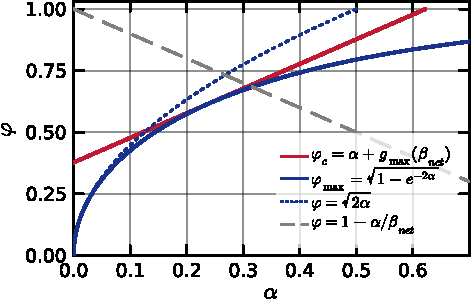
\includegraphics[width=0.45\textwidth]{panels_paper/cusp_vs_extreme.pdf}
\caption{Threshold curves at $\Bnet = 1$. Red straight line:
$\varphi_c(\alpha) = \alpha + g_{\max}(\Bnet)$, tangent to the blue solid curve at the
saddle $\varphi^*(\Bnet)$ (Appendix B). Blue solid:
the exact-density extreme alignment~\eqref{eq:varphi_max}.
Blue dotted: $\sqrt{2\alpha}$, its Gaussian approximation. Grey dashed:
$1 - \alpha/\Bnet$, the \citeauthor{ramsauer2021hopfield} condition.}
\label{fig:varphi}
\end{figure}

The red line is tangent to the blue solid curve at every $\Bnet$; as $\Bnet$
varies, the tangency point sweeps the entire blue solid curve. This follows from
the Legendre conjugacy between $g_{\max}(\Bnet)$ and $\varphi_{\max}(\alpha)$,
derived in Appendix~B. The geometric consequence is that the cusp
$\varphi_c(\alpha, \Bnet)$ lies above the maximum alignment $\varphi_{\max}(\alpha)$
at every $\alpha$: no individual spurious pattern enters the retrieval basin
$\varphi > \varphi_c$. Retrieval loss is therefore \textit{collective}, driven by
the bulk saddle of the spurious sum and not by any single spurious pattern
reaching the target. In the terminology of \citet{lucibello2024exponential}, the
retrieval boundary lies in the \textit{uncondensed} phase of the auxiliary REM,
where exponentially many patterns dominate the noise sum, as opposed to the
\textit{condensed} phase where a single pattern dominates.

\paragraph{Extension to finite temperature.}
At $T > 0$ the entropy density~\citep{icml2026theory}
\begin{equation}
    s(\varphi) = \tfrac{1}{2} \ln(1 - \varphi^2),
    \label{eq:entropy}
\end{equation}
adds to the internal energy, giving the free energy density
$f(\varphi) = u(\varphi) - T\,s(\varphi)$, plotted in Fig.~\ref{fig:cusp} for
$\alpha = 0.5$, $\Bnet = 1$ and several $T$. The profile has two minima: one at
$\varphi \approx 0$ from the spurious sum, one at $\varphi \approx 1$ from the
retrieval term. The retrieval minimum shifts from $\varphi = 1$ at $T = 0$ to
\begin{equation}
    \varphi_{\rm eq}(T) = \tfrac{1}{2}(\sqrt{T^2 + 4} - T)
    \label{eq:phi_eq}
\end{equation}
at $T > 0$, and disappears at the spinodal
$\varphi_{\rm eq}(T) = \varphi_c(\alpha, \Bnet)$, giving
\begin{equation}
    T_{\mathrm{sp}}(\alpha, \Bnet) \;=\; \frac{\Bnet^2 - (\alpha + \gmax(\Bnet))^2}
              {\Bnet\,(\alpha + \gmax(\Bnet))}\,.
    \label{eq:spinodal}
\end{equation}

\begin{figure}[t]
\centering
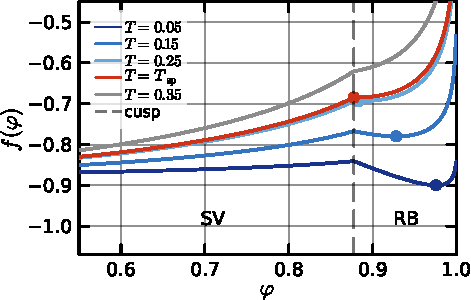
\includegraphics[width=0.45\textwidth]{panels_paper/cusp_illustration.pdf}
\caption{Leading-order free energy density $f(\varphi)$ at $\alpha=0.5$, $\Bnet=1$,
for several $T$. RB: retrieval basin; SV: saddle valley (where the spurious term
dominates); cusp at $\varphi\approx 0.877$ (dashed grey). Coloured dots mark the
RB minima; they disappear at the spinodal temperature
$T_{\rm sp}(\alpha, \Bnet) \approx 0.262$.}
\label{fig:cusp}
\end{figure}

\paragraph{Stability and Kramers escape.}
For $T < T_{\mathrm{sp}}(\alpha, \Bnet)$ the retrieval minimum exists. It is
thermodynamically stable when it is the global minimum of $f$ and metastable when
the saddle-valley minimum is deeper. At equilibrium the deeper basin carries the
larger weight, with the ratio between the two basins set by their depth
difference; at finite $T$ and finite $N$ both basins can carry significant mass.
The chain escapes the retrieval basin to the saddle valley by a Kramers process
at the same rate $\sim \e^{-N \Delta f / T}$ in both
regimes~\citep{kramers1940, hanggi1990}, with $\Delta f$ the per-spin barrier from
the basin minimum to the cusp; what differs is the return rate. A Monte Carlo
ensemble initialised in the basin contains both populations at finite budget, in
proportions set by the budget over the Kramers escape time. As $T \to 0$ the
escape rate vanishes, so retrieval is retained whenever the basin exists.

\section{Monte Carlo schemes}


\section{Results}


\section{Discussion}





% \section{Acknowledgments}


\bibliography{aaai2026}

\appendix

\section{Appendix A: Derivation of the prefactor in the spurious sum}

The integral~\eqref{eq:spur_integral} evaluates in closed form. Substituting
$\varphi = \cos\theta$ maps the spherical density onto the kernel of the integral
representation of the modified Bessel function
$I_\nu(z)$~\citep[8.431.3]{gradshteyn2015}; at $\nu = N/2 - 1$, $z = \Bnet N$,
this gives for $N > 1$
\begin{equation}
S_{\rm spur} = M \Gamma\Big(\tfrac{N}{2}\Big)\left(\frac{2}{\Bnet N}\right)^{\!N/2-1}\!\!\e^{-\Bnet N}\,I_{N/2-1}(\Bnet N).
\label{eq:spurious_exact}
\end{equation}
The right-hand side is the disorder expectation of the sum~\eqref{eq:spur_sum}. The
relative fluctuations of $S_{\rm spur}$ around this expectation are
$\sim \e^{N[\delta(\Bnet) - \alpha]/2}$ with
$\delta(\Bnet) = g_{\max}(2\Bnet) - 2\,g_{\max}(\Bnet) > 0$; they are exponentially
small in $N$ when $\alpha > \delta(\Bnet)$. At $\Bnet = 1$, $\delta \approx 0.334$,
well below the retrieval boundary $\alpha_c \approx 0.623$, so the
saddle~\eqref{eq:spurious_saddle} captures the typical $S_{\rm spur}$.


The Debye uniform asymptotic of the modified Bessel function~\citep[10.41.3]{olver2010nist}
gives the prefactor of~\eqref{eq:spurious_saddle}. Keeping the leading ($k = 0$) term of
the asymptotic series,
\begin{equation}
I_\nu(\nu z') \sim \frac{\e^{\nu\eta(z')}}{(2\pi\nu)^{1/2}(1+{z'}^2)^{1/4}},
\end{equation}
where $z' = 2\Bnet N/(N-2)$ and
\begin{equation}
    \eta(z') = \sqrt{1+{z'}^2} + \ln\frac{z'}{1+\sqrt{1+{z'}^2}}\,.
    \label{eq:bessel_debye}
\end{equation}  
$\eta(z')$ is expanded to $\mathcal{O}(N^{-1})$ because it is multiplied by
$\nu = N/2 - 1$ in the exponent:
\begin{equation}
    \eta(z') = \eta(2\Bnet) + \eta'(2\Bnet) \frac{4\Bnet}{N} + O(N^{-2})\,,
\end{equation}
where
\begin{align}
    \eta(2\Bnet)  &= 1 + 2\Bnet\varphi^* + \ln\varphi^*\,, \\
    \eta'(2\Bnet) &= \varphi^* + \frac{1}{2\Bnet}\,.
\end{align}
Then 
\begin{equation}
    \nu \eta(z') = \tfrac{N}{2} \eta(2\Bnet) - \ln\varphi^* + \mathcal{O}(1/N).
\end{equation}
The $\mathcal{O}(1)$ piece $-\ln\varphi^*$ in the exponent contributes a factor
$1/\varphi^*$ to the prefactor. Using Stirling's formula
\begin{equation}
    \Gamma(N/2) \sim \sqrt{4\pi/N}\,(N/2)^{N/2}\,\e^{-N/2}
\end{equation} 
and collecting all terms in~\eqref{eq:spurious_exact} to $\mathcal{O}(1)$ in the
exponent and to leading order in the prefactor reproduces the exponent
of~\eqref{eq:spurious_saddle} and gives the prefactor:
\begin{equation}
S_{\rm spur} \approx \frac{\e^{N[\alpha + g_{\max}(\Bnet) - \Bnet]}}{\sqrt{1-\varphi^{*4}}}
\label{eq:spurious_laplace}
\end{equation}
with $g_{\max}(\Bnet)$ given by \eqref{eq:saddle_value}.
At $\Bnet = 1$, $\varphi^* \approx 0.618$ and the prefactor is $\approx 1.082$.


\section{Appendix B: Legendre-conjugacy relation between the saddle value and the spherical extreme}

The Legendre transform expresses a duality between two ways of describing a convex
curve: as the graph of a function $y = f(x)$, or as the envelope of its tangent
lines, each labelled by its slope. Legendre introduced it in 1787 to integrate
differential equations by changing the independent variable from a coordinate to
the corresponding slope; the same construction later became central to
thermodynamics (conjugate pairs such as entropy--temperature and volume--pressure)
and to convex optimization (primal--dual duality).

Take the simplest convex curve, the parabola $f(x) = x^2/2$. Its tangent at the
point $(x_0, x_0^2/2)$ has slope $p = x_0$ and $y$-intercept $-x_0^2/2 = -p^2/2$.
Writing the tangent line as $y = p\,x - p^2/2$ and varying $p$, the parabola is
recovered as the upper envelope of this one-parameter family of lines,
\begin{equation}
\tfrac12 x^2 \;=\; \sup_p \bigl[\,p\,x - \tfrac12 p^2\,\bigr],
\end{equation}
with the supremum attained at $p = x$. The same construction defines the Legendre
transform of an arbitrary convex function $f(x)$,
\begin{equation}
f^*(p) \;=\; \sup_x \bigl[\,p\,x - f(x)\,\bigr],
\end{equation}
and the inverse relation $f(x) = \sup_p [p\,x - f^*(p)]$ recovers $f$ as the upper
envelope of its tangent lines indexed by slope. Two convex functions related this
way are called \emph{Legendre conjugates}.

The situation in our problem is exactly this. The spherical extreme
$\varphi_{\max}(\alpha) = \sqrt{1-\e^{-2\alpha}}$, written inversely as
$\alpha = \psi(\varphi)$, takes the form
\begin{equation}
\psi(\varphi) \;=\; -\tfrac12 \ln(1-\varphi^2),
\end{equation}
a convex function on $(-1, 1)$. Its Legendre transform is
\begin{equation}
\psi^*(\Bnet) \;=\; \sup_{\varphi \in (-1, 1)} \bigl[\,\Bnet\,\varphi - \psi(\varphi)\,\bigr].
\end{equation}
The supremum is attained at the spherical saddle
$\varphi = \varphi^*(\Bnet) = (-1 + \sqrt{1+4\Bnet^2})/(2\Bnet)$, the unique
positive root of
\begin{equation}
\Bnet\,\varphi^{*\,2} + \varphi^* - \Bnet = 0.
\end{equation}
Substituting back gives
\begin{equation}
\psi^*(\Bnet) \;=\; \Bnet\,\varphi^* + \tfrac12 \ln(1-\varphi^{*\,2})
\;=\; g_{\max}(\Bnet),
\label{eq:legendre}
\end{equation}
the saddle value~\eqref{eq:saddle_value}. So $g_{\max}$ and $\psi$ are Legendre
conjugates.

The geometric statement of this conjugacy: the cusp line at sharpness $\Bnet$,
\begin{equation}
\varphi_c(\alpha, \Bnet) \;=\; [\alpha + g_{\max}(\Bnet)]/\Bnet,
\end{equation}
is the tangent line to the spherical extreme with slope $1/\Bnet$ and
$\alpha$-intercept $-g_{\max}(\Bnet)$. As $\Bnet$ ranges over $(0, \infty)$, the
family of cusp lines envelopes the spherical extreme from above,
\begin{equation}
\varphi_{\max}(\alpha) \;=\; \inf_{\Bnet > 0} \varphi_c(\alpha, \Bnet),
\end{equation}
with tangency at $\varphi = \varphi^*(\Bnet)$. The geometry of
Fig.~\ref{fig:varphi} is therefore a Legendre duality between the saddle value
$g_{\max}$ on the kernel-sharpness side and the spherical extreme $\varphi_{\max}$
on the alignment side.


\section{Appendix C: Tangency of the cusp lines to the spherical extreme, in figure coordinates}

This appendix shows that the cusp lines
$\varphi_c(\alpha, \Bnet) = (\alpha + g_{\max}(\Bnet))/\Bnet$ are tangent to the
spherical-extreme curve $\varphi_{\max}(\alpha) = \sqrt{1-\e^{-2\alpha}}$ at every
$\Bnet$, that the tangency point sweeps the full curve as $\Bnet$ ranges over
$(0, \infty)$, and that the spherical extreme is the lower envelope of the
cusp-line family. The argument works directly in the $(\alpha, \varphi)$
coordinates of Fig.~\ref{fig:varphi}: $\alpha$ on the x-axis, $\varphi$ on the
y-axis. It splits into two steps: matching the slope of the tangent to the blue
curve with the slope of the cusp line, which gives parallelism, and matching the
y-intercept, which upgrades parallelism to coincidence. The slope step pulls out
the saddle equation; the intercept step expresses the Legendre conjugacy of
$g_{\max}$ and $\varphi_{\max}$.

\paragraph{Concavity of the blue curve.}
Differentiating $\varphi_{\max}(\alpha) = \sqrt{1-\e^{-2\alpha}}$ once gives
\begin{equation}
\varphi_{\max}'(\alpha) \;=\; \frac{1-\varphi_{\max}^2}{\varphi_{\max}},
\label{eq:tangent_slope_C}
\end{equation}
and a second differentiation gives $\varphi_{\max}''(\alpha) < 0$ for $\alpha > 0$,
so $\varphi_{\max}$ is strictly concave on $(0, \infty)$. For a concave function
every tangent line lies above the function, with equality only at the tangency
point. This will give the lower-envelope identity at the end.

\paragraph{Step A: matching the slope (parallelism).}
The cusp line at sharpness $\Bnet$,
\begin{equation}
\varphi \;=\; \alpha/\Bnet + g_{\max}(\Bnet)/\Bnet,
\end{equation}
has slope $1/\Bnet$ and y-intercept $g_{\max}(\Bnet)/\Bnet$. To find the point on
the blue curve where the tangent has the same slope, set the right-hand side
of~\eqref{eq:tangent_slope_C} equal to $1/\Bnet$:
\begin{equation}
\frac{1-\varphi^2}{\varphi} \;=\; \frac{1}{\Bnet}
\quad\Longleftrightarrow\quad
\Bnet\,\varphi^2 + \varphi - \Bnet = 0.
\label{eq:saddle_eq_C}
\end{equation}
This is the saddle equation; its unique positive root is the spherical saddle
\begin{equation}
\varphi^*(\Bnet) \;=\; \frac{-1 + \sqrt{1+4\Bnet^2}}{2\Bnet}.
\end{equation}
The corresponding $\alpha$ on the blue curve follows from
$\varphi^* = \varphi_{\max}(\alpha^*)$, that is, $\e^{-2\alpha^*} = 1 - \varphi^{*\,2}$:
\begin{equation}
\alpha^*(\Bnet) \;=\; -\tfrac12 \ln(1-\varphi^{*\,2}).
\label{eq:alpha_star_C}
\end{equation}
At the point $(\alpha^*(\Bnet), \varphi^*(\Bnet))$ on the blue curve, the tangent
has slope $1/\Bnet$, equal to the slope of the cusp line. Step~A establishes
\textit{parallelism} between the tangent at this point and the cusp line; it does
not yet show the two lines coincide.

\paragraph{Step B: matching the y-intercept (coincidence).}
A line of slope $1/\Bnet$ passing through $(\alpha^*(\Bnet), \varphi^*(\Bnet))$ has
y-intercept
\begin{equation}
b_{\rm tangent}(\Bnet) \;=\; \varphi^* - \alpha^*/\Bnet.
\end{equation}
The cusp line has y-intercept $g_{\max}(\Bnet)/\Bnet$. Using the definition
$g_{\max}(\Bnet) = g(\varphi^*, \Bnet) = \tfrac12 \ln(1-\varphi^{*\,2}) + \Bnet\,\varphi^*$
from~\eqref{eq:saddle_value} together with $\alpha^* = -\tfrac12 \ln(1-\varphi^{*\,2})$
from~\eqref{eq:alpha_star_C}, the cusp-line intercept becomes
\begin{equation}
\frac{g_{\max}(\Bnet)}{\Bnet}
\;=\; \frac{\tfrac12 \ln(1-\varphi^{*\,2})}{\Bnet} + \varphi^*
\;=\; -\frac{\alpha^*(\Bnet)}{\Bnet} + \varphi^*
\;=\; b_{\rm tangent}(\Bnet).
\label{eq:intercept_match_C}
\end{equation}
The y-intercepts coincide. Two lines with the same slope and the same y-intercept
are the same line. The cusp line at sharpness $\Bnet$ therefore coincides with
the tangent to the blue curve at $(\alpha^*(\Bnet), \varphi^*(\Bnet))$ — two
independently defined lines, one set by the energy landscape and one by the
geometry of $\varphi_{\max}$, turn out to be the same line.

\paragraph{Lower envelope.}
By the concavity statement at the start of this appendix, every tangent line lies
above the blue curve, with equality only at the tangency point. So the cusp line
at any sharpness $\Bnet$ lies above the blue curve, with equality only at
$\alpha = \alpha^*(\Bnet)$:
\begin{equation}
\varphi_c(\alpha, \Bnet) \;\ge\; \varphi_{\max}(\alpha) \quad \text{for all $\alpha$ and all $\Bnet > 0$},
\end{equation}
with equality at one $\alpha$ for each $\Bnet$. Taking the infimum over $\Bnet$,
\begin{equation}
\varphi_{\max}(\alpha) \;=\; \inf_{\Bnet > 0} \varphi_c(\alpha, \Bnet),
\label{eq:lower_envelope_C}
\end{equation}
the lower envelope identity in figure coordinates.

\paragraph{Tangency sweeps the blue curve.}
The map $\Bnet \mapsto \varphi^*(\Bnet)$ is continuous and strictly increasing on
$(0, \infty)$, with $\varphi^*(\Bnet) \to 0$ as $\Bnet \to 0^+$ and
$\varphi^*(\Bnet) \to 1$ as $\Bnet \to \infty$. As $\Bnet$ sweeps $(0, \infty)$,
the tangency point $(\alpha^*(\Bnet), \varphi^*(\Bnet))$ therefore traces the
entire blue curve from the origin to its right edge.

\paragraph{Where the Legendre transform sits.}
The cusp line at sharpness $\Bnet$ and the tangent to the blue curve of slope
$1/\Bnet$ are two independently defined objects. The cusp line comes from the
energy landscape via the saddle value $g_{\max}(\Bnet)$; the tangent comes from
the geometry of the spherical extreme. The y-intercept of either, expressed as a
function of $\Bnet$, is the (concave) Legendre transform of $\varphi_{\max}$:
\begin{equation}
g_{\max}(\Bnet)/\Bnet \;=\; \sup_\alpha\,\bigl[\,\varphi_{\max}(\alpha) - \alpha/\Bnet\,\bigr],
\end{equation}
with the supremum attained at $\alpha = \alpha^*(\Bnet)$, where the slope-match
condition~\eqref{eq:saddle_eq_C} holds. Two lines with the same slope and the
same y-intercept are the same line; the Legendre identity therefore expresses
the coincidence of the cusp line at $\Bnet$ with the tangent line of slope
$1/\Bnet$. The lower-envelope identity~\eqref{eq:lower_envelope_C} is the
inverse statement: the spherical extreme is recovered as the lower envelope of
the cusp lines parameterised by sharpness $\Bnet$.


\end{document}
